\documentclass[12pt, a4paper]{report}
\usepackage[top=1cm, left=1cm, right=1cm]{geometry}

\usepackage[utf8]{inputenc}
\usepackage[russian]{babel}

\usepackage{array}
\newcolumntype{M}[1]{>{\centering\arraybackslash}m{#1}}

\usepackage{hyperref}
\hypersetup{
	colorlinks,
	citecolor=black,
	filecolor=black,
	linkcolor=black,
	urlcolor=black
}

\usepackage{sectsty}
\allsectionsfont{\centering}

\usepackage{indentfirst}
\setlength\parindent{24pt}

\usepackage{algorithm}
\usepackage[noend]{algpseudocode}

\usepackage{listings}
\usepackage{xcolor}
\definecolor{codegreen}{rgb}{0,0.6,0}
\definecolor{codegray}{rgb}{0.5,0.5,0.5}
\definecolor{codepurple}{rgb}{0.58,0,0.82}
\definecolor{backcolour}{rgb}{0.95,0.95,0.92}
\lstdefinestyle{mystyle}{
    backgroundcolor=\color{backcolour},   
    commentstyle=\color{codegreen},
    keywordstyle=\color{magenta},
    numberstyle=\normalsize\color{codegray},
    stringstyle=\color{codepurple},
    basicstyle=\ttfamily\footnotesize,
    breakatwhitespace=false,         
    breaklines=true,                 
    captionpos=b,                    
    keepspaces=true,                 
    numbers=left,                    
    numbersep=5pt,                  
    showspaces=false,                
    showstringspaces=false,
    showtabs=false,                  
    tabsize=2
}

\usepackage{graphicx}
\graphicspath{{plots/pictures/}}

\begin{document}
	\begin{titlepage}
		\begin{center}
			\large \textbf{Министерство науки и высшего образования Российской Федерации} \\
			\large \textbf{Федеральное государственное бюджетное образовательное учреждение высшего образования} \\
			\large \textbf{«Российский химико-технологический университет имени Д.И. Менделеева»} \\

			\vspace*{4cm}
			\LARGE \textbf{ОТЧЕТ ПО ЛАБОРАТОРНОЙ РАБОТЕ №2}

			\vspace*{4cm}
			\begin{flushright}
				\Large
				\begin{tabular}{>{\raggedleft\arraybackslash}p{9cm} p{10cm}}
					Выполнил студент группы КС-36: & Золотухин А.А. \\
					Ссылка на репозиторий: & https://github.com/ \\ 
					& CorgiPuppy/ \\
					& parallel-prog-labs \\
					Принял: & Бабкин Михаил Андреевич \\
					Дата сдачи: & 01.10.2025 \\
				\end{tabular}

			\end{flushright}

			\vspace*{6cm}
			\Large \textbf{Москва \\ 2025}
		\end{center}
	\end{titlepage}
	
	\tableofcontents	
	\thispagestyle{empty}
	\newpage

	\pagenumbering{arabic}
	
	\section*{Описание задачи}
	\addcontentsline{toc}{section}{Описание задачи}
	\large
	Найти скалярное произведение векторов \textit{A} и \textit{B}, заполненных случайными целыми числами от \underline{0} до \underline{100}. Длина векторов выбирается из множества {\underline{10000}; \underline{100000}; \underline{1000000}; \underline{10000000}} (рассмотреть \underline{4} случая). Использовать \underline{10} потоков. Измерить время работы программы в каждом случае, построить график зависимости времени выполнения от длины вектора.	
	\section*{Выполнение задачи}
	\addcontentsline{toc}{section}{Выполнение задачи}
	\large

	\lstset{style=mystyle}
	\lstinputlisting[language=C++]{src/main.cpp}

	\begin{center}
		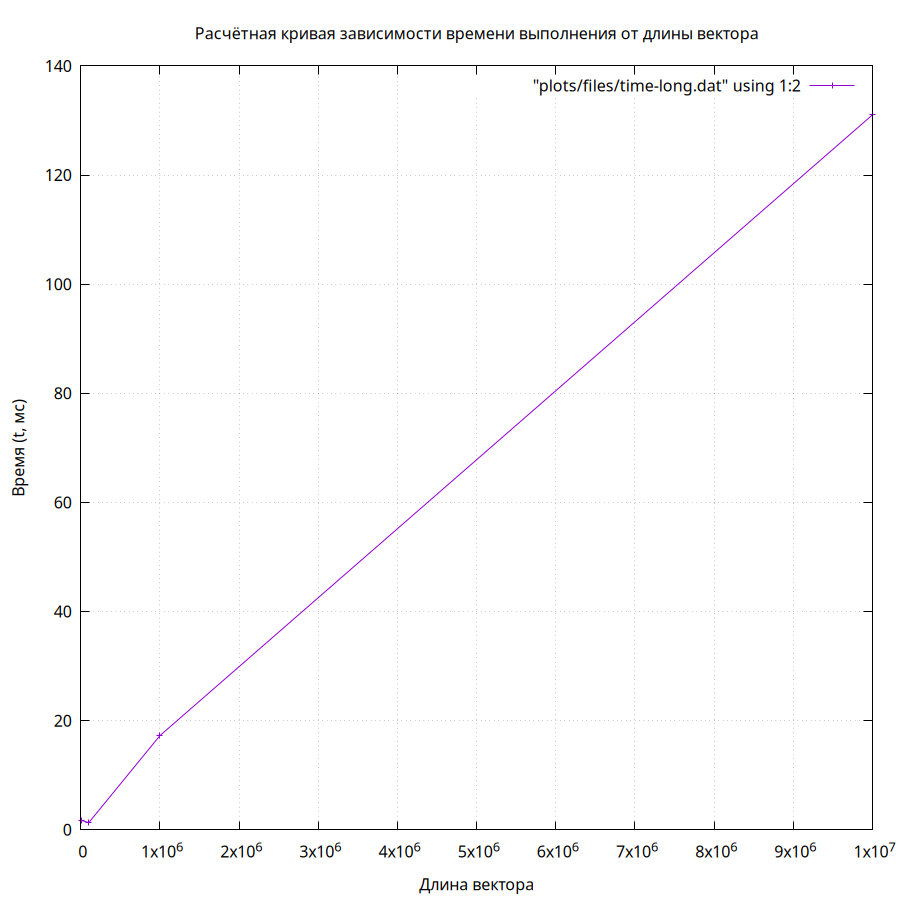
\includegraphics[width=500pt]{time-long.png}
	\end{center}
\end{document}
